\chapter{Ports and Adapters Architecture}

\section{Pendahuluan}

Dalam pengembangan perangkat lunak, pemilihan arsitektur yang tepat menjadi salah satu faktor penentu keberhasilan sebuah aplikasi. Arsitektur yang baik memungkinkan aplikasi untuk tetap fleksibel, dapat diperluas, dan mudah dipelihara seiring perkembangan teknologi dan kebutuhan bisnis. Salah satu tantangan utama dalam pengembangan aplikasi adalah mengelola ketergantungan antara berbagai komponen, terutama antara logika bisnis dan teknologi eksternal seperti database, API, dan antarmuka pengguna.

Hexagonal Architecture, atau yang dikenal sebagai \textbf{Ports and Adapters Architecture}, adalah pendekatan yang dirancang untuk mengatasi tantangan ini. Dengan memisahkan logika bisnis inti dari teknologi eksternal, arsitektur ini memberikan fleksibilitas yang lebih besar dalam perubahan sistem, memungkinkan pengujian yang lebih mudah, serta meningkatkan modularitas aplikasi. Arsitektur ini pertama kali diperkenalkan oleh \textbf{Alistair Cockburn} pada tahun 2005 dan sejak saat itu telah menjadi salah satu pola yang banyak digunakan dalam pengembangan perangkat lunak modern.

Dokumen ini membahas konsep, prinsip, dan implementasi \textbf{Hexagonal Architecture} dalam bahasa pemrograman \textbf{Java}. Melalui pendekatan ini, pengembang dapat membangun aplikasi yang lebih terstruktur, terisolasi dari perubahan teknologi, dan lebih mudah diuji serta dipelihara.

\section{Latar Belakang}

Dalam pengembangan perangkat lunak, arsitektur aplikasi memiliki peran penting dalam menentukan bagaimana komponen-komponen di dalamnya berinteraksi. Arsitektur tradisional, seperti \textit{layered architecture} (n-tier architecture), sering kali menghasilkan ketergantungan yang kuat antara lapisan-lapisannya. Misalnya, perubahan dalam lapisan penyimpanan data dapat berdampak langsung pada lapisan logika bisnis dan presentasi, sehingga menyulitkan perawatan dan pengembangan lebih lanjut.

Untuk mengatasi masalah tersebut, berbagai pendekatan arsitektur perangkat lunak yang lebih fleksibel dan modular telah dikembangkan. Salah satu pendekatan yang muncul adalah \textbf{Hexagonal Architecture}, yang juga dikenal sebagai \textit{Ports and Adapters Architecture}. Konsep ini pertama kali diperkenalkan oleh \textbf{Alistair Cockburn} pada tahun 2005 dengan tujuan utama memisahkan logika bisnis inti dari teknologi eksternal, seperti database, API, dan antarmuka pengguna. Dengan pendekatan ini, perubahan pada salah satu komponen tidak akan berdampak langsung pada komponen lainnya.

\subsection{Sejarah Hexagonal Architecture}

Hexagonal Architecture lahir dari kebutuhan untuk menciptakan perangkat lunak yang lebih \textit{modular}, mudah diuji, dan fleksibel terhadap perubahan teknologi. Pada awal tahun 2000-an, banyak aplikasi monolitik memiliki ketergantungan yang kuat terhadap framework dan teknologi spesifik, yang menyebabkan kesulitan dalam melakukan migrasi atau perubahan arsitektur.

Alistair Cockburn memperkenalkan konsep ini dengan gagasan utama bahwa logika bisnis inti harus diisolasi dari dunia luar melalui \textbf{ports} (antarmuka komunikasi) dan \textbf{adapters} (implementasi yang memungkinkan komunikasi dengan teknologi eksternal). Dengan struktur ini, suatu aplikasi dapat dengan mudah diuji menggunakan \textit{mock} atau \textit{stub} tanpa bergantung pada teknologi seperti database atau layanan eksternal lainnya.

Konsep ini kemudian mendapat lebih banyak perhatian seiring berkembangnya praktik \textbf{Clean Architecture} yang diperkenalkan oleh \textbf{Robert C. Martin} (Uncle Bob) serta pendekatan berbasis \textbf{Domain-Driven Design (DDD)} yang dipopulerkan oleh \textbf{Eric Evans}. Hingga saat ini, Hexagonal Architecture banyak diadopsi dalam pengembangan aplikasi modern, terutama pada sistem yang membutuhkan fleksibilitas tinggi dalam mengintegrasikan berbagai teknologi.

\subsection{Motivasi Penggunaan Hexagonal Architecture}

Beberapa alasan utama mengapa Hexagonal Architecture semakin banyak digunakan dalam pengembangan perangkat lunak adalah sebagai berikut:

\begin{itemize}
	\item \textbf{Memisahkan logika bisnis dari ketergantungan teknologi} \\
	Dengan adanya \textit{ports and adapters}, perubahan pada teknologi penyimpanan data, framework, atau sistem eksternal lainnya tidak berdampak langsung pada domain bisnis.
	
	\item \textbf{Memudahkan pengujian unit dan integrasi} \\
	Karena tidak ada ketergantungan langsung dengan teknologi eksternal, pengujian dapat dilakukan secara independen tanpa memerlukan koneksi ke database atau layanan eksternal.
	
	\item \textbf{Fleksibilitas dalam penggantian teknologi} \\
	Dengan pendekatan ini, tim pengembang dapat mengganti database, sistem pesan, atau antarmuka pengguna tanpa harus mengubah logika bisnis yang sudah ada.
	
	\item \textbf{Struktur yang lebih modular dan mudah dikembangkan} \\
	Arsitektur ini memudahkan pengembang dalam menambahkan fitur baru atau mengganti bagian dari sistem tanpa merusak keseluruhan sistem.
\end{itemize}

Dengan semua manfaat tersebut, Hexagonal Architecture menjadi solusi yang kuat untuk membangun perangkat lunak yang \textbf{fleksibel}, \textbf{dapat dipelihara}, dan \textbf{mudah diuji}.


\section{Definisi, Prinsip, dan Struktur Hexagonal Architecture}

Hexagonal Architecture, yang juga dikenal sebagai \textit{Ports and Adapters Architecture}, adalah pola arsitektur perangkat lunak yang bertujuan untuk memisahkan logika bisnis inti dari teknologi eksternal seperti database, API, dan antarmuka pengguna. Konsep ini memungkinkan fleksibilitas dalam mengubah teknologi yang digunakan tanpa perlu mengubah logika inti aplikasi.

Pendekatan ini didasarkan pada ide bahwa sebuah sistem harus memiliki antarmuka yang jelas dalam berkomunikasi dengan dunia luar. Hal ini dicapai melalui penggunaan \textbf{ports} (antarmuka komunikasi) dan \textbf{adapters} (implementasi yang memungkinkan interaksi dengan teknologi eksternal). Dengan demikian, komponen dalam aplikasi tidak memiliki ketergantungan langsung terhadap teknologi spesifik.

\subsection{Prinsip Hexagonal Architecture}

Hexagonal Architecture memiliki beberapa prinsip utama yang menjadi dasar penerapannya:

\begin{itemize}
	\item \textbf{Pemisahan Logika Bisnis dan Teknologi Eksternal} \\
	Logika bisnis diletakkan di bagian inti (\textit{domain}) aplikasi, sementara detail teknis seperti database, layanan eksternal, dan antarmuka pengguna hanya berinteraksi melalui \textit{ports and adapters}.
	
	\item \textbf{Interaksi Melalui Ports dan Adapters} \\
	Semua interaksi antara domain bisnis dan dunia luar dilakukan melalui \textit{ports} (interface yang mendefinisikan kontrak komunikasi) dan \textit{adapters} (implementasi dari ports yang berkomunikasi dengan teknologi tertentu).
	
	\item \textbf{Dukungan terhadap Pengujian yang Lebih Mudah} \\
	Dengan struktur ini, unit bisnis dapat diuji secara independen tanpa harus bergantung pada database atau sistem eksternal lainnya. Hal ini memungkinkan penggunaan \textit{mock} atau \textit{stub} dalam pengujian.
	
	\item \textbf{Fleksibilitas dalam Perubahan Teknologi} \\
	Karena teknologi eksternal hanya dihubungkan melalui adapters, mengganti database, framework, atau layanan eksternal lainnya dapat dilakukan tanpa mengubah logika inti aplikasi.
\end{itemize}

\subsection{Struktur Hexagonal Architecture}

Gambar \ref{fig:hexagonal_architecture} menunjukkan bagaimana komponen-komponen dalam Hexagonal Architecture saling berinteraksi:

\begin{figure}[h]
	\centering
	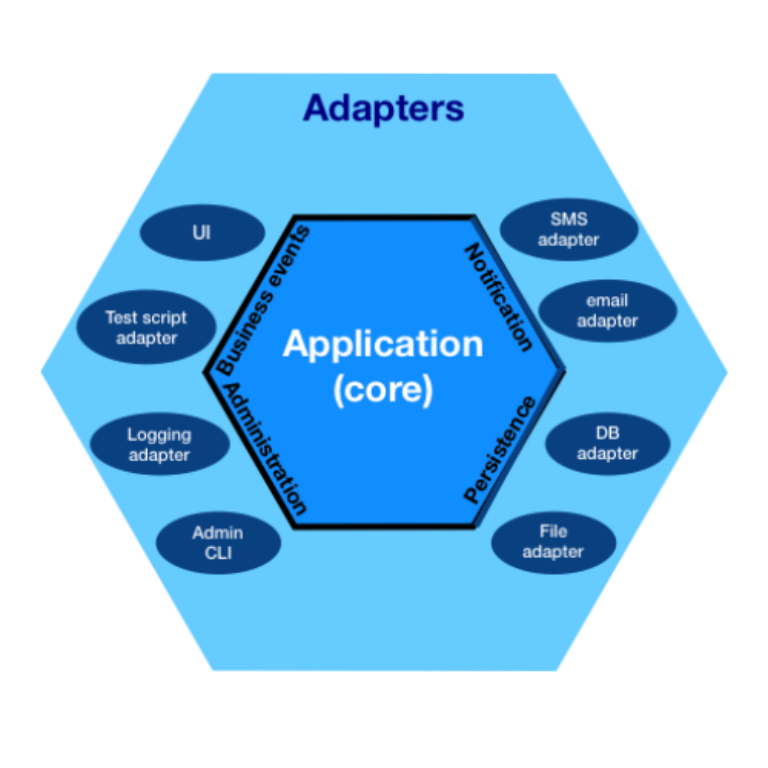
\includegraphics[width=.8\textwidth]{../images/hexagonal_architecture.png}
	\caption{Hexagonal Architecture}
	\label{fig:hexagonal_architecture}
\end{figure}

Hexagonal Architecture membagi sistem menjadi tiga bagian utama:

\begin{enumerate}
	\item \textbf{Domain} \\
	Domain merupakan inti dari aplikasi yang berisi logika bisnis utama. Bagian ini harus bebas dari ketergantungan terhadap teknologi eksternal agar tetap bersifat murni (\textit{pure business logic}).
	
	\item \textbf{Ports} \\
	Ports adalah antarmuka yang menghubungkan domain dengan dunia luar. Ports mendefinisikan kontrak komunikasi yang digunakan oleh adapters untuk berinteraksi dengan domain.
	
	\item \textbf{Adapters} \\
	Adapters adalah implementasi dari ports yang memungkinkan interaksi dengan teknologi eksternal, seperti database, sistem pesan, atau antarmuka pengguna. Adapters bertanggung jawab untuk menerjemahkan data dari format eksternal ke format yang dapat dipahami oleh domain.
\end{enumerate}




\section{Kelebihan Hexagonal Architecture}

Hexagonal Architecture memiliki berbagai keunggulan dalam pengembangan perangkat lunak, terutama dalam hal modularitas, kemudahan pengujian, dan fleksibilitas terhadap perubahan teknologi. Berikut adalah beberapa kelebihan utama dari pendekatan ini:

\begin{enumerate}
	\item \textbf{Pemisahan Logika Bisnis dan Teknologi Eksternal} \\
	Logika bisnis ditempatkan di dalam \textit{domain}, sementara interaksi dengan teknologi eksternal seperti database, API, atau sistem pesan hanya dilakukan melalui \textit{ports} dan \textit{adapters}. Hal ini memastikan bahwa perubahan pada teknologi eksternal tidak berdampak langsung pada logika bisnis utama.
	
	\item \textbf{Memudahkan Pengujian Unit dan Integrasi} \\
	Karena domain tidak memiliki ketergantungan langsung terhadap teknologi eksternal, pengujian dapat dilakukan secara mandiri menggunakan \textit{mock} atau \textit{stub}. Dengan demikian, pengembang dapat menguji logika bisnis tanpa perlu bergantung pada infrastruktur seperti database atau layanan eksternal lainnya, sehingga meningkatkan kecepatan dan efektivitas pengujian.
	
	\item \textbf{Fleksibilitas dalam Penggantian Teknologi} \\
	Dengan adanya lapisan \textit{adapters}, teknologi yang digunakan di sisi luar domain dapat diganti tanpa mengubah kode dalam logika bisnis. Misalnya, jika sebuah aplikasi awalnya menggunakan MySQL sebagai penyimpanan data dan kemudian ingin beralih ke PostgreSQL atau MongoDB, perubahan tersebut dapat dilakukan dengan hanya mengganti implementasi adapter tanpa perlu mengubah domain atau layanan bisnis yang sudah ada.
	
	\item \textbf{Struktur yang Modular dan Mudah Dikembangkan} \\
	Dengan membagi aplikasi menjadi domain, ports, dan adapters, sistem menjadi lebih terorganisir dan mudah diperluas. Setiap komponen dapat dikembangkan secara independen, memungkinkan tim pengembang untuk bekerja secara paralel tanpa mengganggu bagian lain dari aplikasi.
	
	\item \textbf{Mendukung Prinsip Pemrograman yang Baik} \\
	Hexagonal Architecture mengikuti prinsip-prinsip pemrograman yang baik, seperti \textit{Separation of Concerns} (SoC) dan \textit{Dependency Inversion Principle} (DIP) dari SOLID. Dengan mengikuti prinsip-prinsip ini, kode menjadi lebih bersih, lebih terstruktur, dan lebih mudah dipahami serta dipelihara.
\end{enumerate}

Dengan semua keunggulan ini, Hexagonal Architecture menjadi pilihan yang ideal bagi pengembangan sistem yang membutuhkan fleksibilitas, skalabilitas, dan kemudahan pemeliharaan dalam jangka panjang.

\section{Kekurangan Hexagonal Architecture}

Meskipun Hexagonal Architecture memiliki banyak keunggulan, pendekatan ini juga memiliki beberapa kekurangan yang perlu dipertimbangkan sebelum diterapkan. Berikut adalah beberapa tantangan utama yang dapat dihadapi:

\begin{enumerate}
	\item \textbf{Kompleksitas Tambahan dalam Desain} \\
	Hexagonal Architecture memperkenalkan lapisan tambahan seperti \textit{ports} dan \textit{adapters}, yang meningkatkan kompleksitas desain sistem. Pengembang harus memahami cara menerapkan pola ini dengan benar agar manfaatnya dapat dimaksimalkan tanpa menambah beban yang tidak perlu.
	
	\item \textbf{Membutuhkan Lebih Banyak Kode} \\
	Dengan adanya pemisahan antara domain, ports, dan adapters, jumlah kode yang harus ditulis menjadi lebih banyak dibandingkan dengan arsitektur tradisional. Hal ini dapat memperpanjang waktu pengembangan dan meningkatkan beban pemeliharaan.
	
	\item \textbf{Kurva Belajar yang Lebih Curam} \\
	Pengembang yang belum familiar dengan konsep Hexagonal Architecture mungkin akan mengalami kesulitan dalam memahami cara kerja dan penerapannya. Dibutuhkan waktu untuk mempelajari dan mengadopsi pendekatan ini secara efektif.
	
	\item \textbf{Tidak Selalu Cocok untuk Aplikasi Sederhana} \\
	Untuk aplikasi kecil dengan kebutuhan bisnis yang sederhana, Hexagonal Architecture mungkin dianggap terlalu berlebihan. Struktur tambahan yang diperkenalkan dapat menjadi beban daripada keuntungan dalam proyek dengan kompleksitas rendah.
	
	\item \textbf{Meningkatkan Overhead dalam Komunikasi Antar Komponen} \\
	Karena setiap interaksi antara domain dan teknologi eksternal harus melalui ports dan adapters, ada potensi peningkatan overhead dalam komunikasi antar komponen dibandingkan dengan arsitektur yang lebih langsung.
\end{enumerate}

Meskipun memiliki beberapa kekurangan, Hexagonal Architecture tetap menjadi pilihan yang baik dalam pengembangan perangkat lunak yang membutuhkan fleksibilitas tinggi, kemudahan pengujian, dan skalabilitas jangka panjang.



\section{Contoh Implementasi dalam Java}

Untuk memahami bagaimana Hexagonal Architecture dapat diterapkan dalam pengembangan perangkat lunak menggunakan Java, berikut adalah contoh implementasi dengan studi kasus manajemen pengguna. Implementasi ini mencakup tiga komponen utama dalam Hexagonal Architecture: \textit{Domain}, \textit{Adapters}, dan layanan aplikasi.



\subsection{Definisi Domain}

Bagian \textbf{domain} merupakan inti dari sistem yang berisi logika bisnis utama. Domain harus dibuat sedemikian rupa sehingga tidak memiliki ketergantungan terhadap teknologi eksternal, seperti database, framework, atau sistem antarmuka pengguna. Dengan pendekatan ini, logika bisnis tetap bersifat murni (\textit{pure business logic}) dan dapat digunakan kembali tanpa bergantung pada detail implementasi teknis.

Domain dalam studi kasus ini adalah sistem manajemen akun pelanggan, yang mencakup validasi akun, pemrosesan saldo, dan transaksi pelanggan.

\begin{enumerate}
	\item \textbf{Entitas (\textit{Entity})} \\
	Entitas utama dalam domain ini adalah \texttt{CustomerAccount}, yang merepresentasikan akun pelanggan dengan fitur seperti ID unik, nama pelanggan, saldo akun, serta operasi bisnis seperti melakukan deposit dan penarikan saldo.
	
	\begin{lstlisting}[style=JavaStyle, caption=CustomerAccount Entity]
		public class CustomerAccount {
			private String id;
			private String name;
			private double balance;
			
			public CustomerAccount(String id, String name, double initialBalance) {
				if (initialBalance < 0) {
					throw new IllegalArgumentException("Saldo awal tidak boleh negatif.");
				}
				this.id = id;
				this.name = name;
				this.balance = initialBalance;
			}
			
			public String getId() { return id; }
			public String getName() { return name; }
			public double getBalance() { return balance; }
			
			public void deposit(double amount) {
				if (amount <= 0) {
					throw new IllegalArgumentException("Jumlah deposit harus lebih dari nol.");
				}
				this.balance += amount;
			}
			
			public void withdraw(double amount) {
				if (amount <= 0) {
					throw new IllegalArgumentException("Jumlah penarikan harus lebih dari nol.");
				}
				if (amount > this.balance) {
					throw new IllegalArgumentException("Saldo tidak mencukupi untuk penarikan.");
				}
				this.balance -= amount;
			}
		}
	\end{lstlisting}

	\begin{itemize}
		\item Kelas \texttt{CustomerAccount} merepresentasikan akun pelanggan dengan tiga atribut utama:
		\begin{itemize}
			\item \texttt{id}: ID unik pelanggan.
			\item \texttt{name}: Nama pelanggan.
			\item \texttt{balance}: Saldo akun pelanggan.
		\end{itemize}
		\item Konstruktor memastikan bahwa saldo awal tidak boleh negatif.
		\item Metode \texttt{deposit(double amount)} digunakan untuk menambahkan dana ke akun pelanggan dengan validasi jumlah yang harus lebih dari nol.
		\item Metode \texttt{withdraw(double amount)} memastikan bahwa pelanggan hanya dapat menarik saldo jika jumlahnya mencukupi dan lebih dari nol.
		\item Semua operasi dilakukan di dalam domain tanpa ketergantungan pada teknologi eksternal.
	\end{itemize}
	
	\item \textbf{Logika Bisnis ada di Domain} \\
	Dalam pendekatan Hexagonal Architecture, domain bertanggung jawab atas logika bisnis utama untuk menjaga isolasi dari teknologi eksternal. Beberapa alasan utama mengapa logika bisnis harus ditempatkan di domain adalah:
	\begin{itemize}
		\item Memastikan aturan bisnis tetap konsisten di seluruh aplikasi, terlepas dari teknologi yang digunakan.
		\item Memudahkan pengujian unit karena logika bisnis dapat diuji secara independen tanpa ketergantungan pada database atau antarmuka pengguna.
		\item Memungkinkan fleksibilitas dalam perubahan sistem tanpa harus mengubah keseluruhan arsitektur.
	\end{itemize}
\end{enumerate}

Dengan struktur ini, domain tetap fleksibel, modular, dan dapat digunakan kembali dalam berbagai skenario tanpa bergantung pada detail teknis tertentu.


\subsection{Definisi Port}

Dalam Hexagonal Architecture, \textbf{port} adalah antarmuka yang mendefinisikan bagaimana komponen domain berinteraksi dengan dunia luar, seperti layanan database, sistem eksternal, atau antarmuka pengguna. Port bertindak sebagai jembatan yang memungkinkan komunikasi antara domain dan teknologi eksternal tanpa menciptakan ketergantungan langsung terhadap implementasi spesifik.

\begin{enumerate}
	\item \textbf{Peran Port dalam Hexagonal Architecture} \\
	Port memiliki peran penting dalam menjaga modularitas dan fleksibilitas arsitektur, dengan beberapa fungsi utama:
	\begin{itemize}
		\item \textbf{Memisahkan logika bisnis dari teknologi eksternal} – Domain tidak perlu mengetahui detail teknis tentang bagaimana data disimpan atau bagaimana layanan lain bekerja.
		\item \textbf{Mendefinisikan kontrak komunikasi} – Port menentukan antarmuka yang harus diimplementasikan oleh teknologi eksternal, seperti database atau API.
		\item \textbf{Mempermudah pengujian unit} – Dengan menggunakan port, pengujian dapat dilakukan menggunakan \textit{mock} atau \textit{stub} tanpa bergantung pada implementasi nyata.
		\item \textbf{Memungkinkan perubahan teknologi tanpa mempengaruhi domain} – Jika teknologi penyimpanan data berubah (misalnya dari MySQL ke MongoDB), hanya adapter yang perlu diubah tanpa mempengaruhi logika bisnis.
	\end{itemize}
	
	\item \textbf{Jenis Port dalam Hexagonal Architecture} \\
	Dalam implementasi Hexagonal Architecture, terdapat dua jenis utama port:
	
	\begin{itemize}
		\item \textbf{Inbound Port (Driving Port)} \\
		Port ini digunakan untuk menerima permintaan dari luar dan meneruskannya ke domain. Contohnya adalah layanan API atau antarmuka pengguna yang memicu tindakan dalam domain.
		
		\item \textbf{Outbound Port (Driven Port)} \\
		Port ini digunakan oleh domain untuk berkomunikasi dengan dunia luar, seperti database atau layanan eksternal. Domain memanggil port ini, tetapi implementasinya ditentukan oleh adapter.
	\end{itemize}
	
	\item \textbf{Contoh Implementasi Port dalam Java} \\
	Dalam studi kasus manajemen akun pelanggan, kita mendefinisikan port untuk menghubungkan domain dengan lapisan penyimpanan data. Port ini memungkinkan domain menyimpan dan mengambil data pelanggan tanpa mengetahui detail teknis dari database.
	
	\begin{lstlisting}[style=JavaStyle, caption=CustomerAccountRepository Port]
		public interface CustomerAccountRepository {
			void save(CustomerAccount account);
			CustomerAccount findById(String id);
		}
	\end{lstlisting}
	
	\textbf{Penjelasan:}
	\begin{itemize}
		\item \texttt{CustomerAccountRepository} adalah port yang mendefinisikan kontrak untuk penyimpanan akun pelanggan.
		\item Metode \texttt{save(CustomerAccount account)} digunakan untuk menyimpan atau memperbarui akun pelanggan.
		\item Metode \texttt{findById(String id)} digunakan untuk mengambil akun pelanggan berdasarkan ID.
		\item Implementasi dari antarmuka ini akan dibuat dalam adapter yang berinteraksi dengan database.
	\end{itemize}
\end{enumerate}

Dengan pendekatan ini, domain tetap independen dari teknologi penyimpanan data. Jika di masa depan aplikasi ingin mengganti database dari SQL ke NoSQL, kita hanya perlu mengubah implementasi adapter tanpa menyentuh domain atau layanan bisnis yang sudah ada.


\subsection{Implementasi Adapter}

Dalam Hexagonal Architecture, \textbf{adapter} bertanggung jawab untuk menghubungkan domain dengan teknologi eksternal, seperti database. Adapter ini mengimplementasikan \textit{port} yang telah didefinisikan sebelumnya, yaitu \texttt{CustomerAccountRepository}, sehingga domain tetap bebas dari ketergantungan terhadap detail teknis penyimpanan data.

Pada implementasi ini, kita akan membuat dua adapter berbeda untuk mendukung dua jenis database: \textbf{MySQL} dan \textbf{PostgreSQL}. Keduanya akan mengimplementasikan port yang sama, sehingga domain tidak perlu mengetahui perbedaan di antara keduanya.

\begin{enumerate}
	\item \textbf{Implementasi Adapter untuk MySQL}
	
	Adapter ini menggunakan JDBC untuk berinteraksi dengan MySQL. Implementasi adapter MySQL dapat dilihat pada \ref{lst:mysql_adapter}. Kelas \texttt{MySQLCustomerAccountRepository} mengimplementasikan port \texttt{CustomerAccountRepository}, yang bertindak sebagai antarmuka antara domain bisnis dan database. Kelas ini menangani penyimpanan dan pengambilan data pelanggan dengan metode yang telah ditentukan dalam antarmuka.
	
	\begin{lstlisting}[style=JavaStyle, caption=MySQL Adapter Implementation, label=lst:mysql_adapter]
		public class MySQLCustomerAccountRepository implements CustomerAccountRepository {
			private Connection connection;
			
			// Konstruktor yang secara otomatis membuat koneksi ke database MySQL
			public MySQLCustomerAccountRepository() throws SQLException {
				this.connection = DriverManager.getConnection(
				"jdbc:mysql://localhost:3306/customer_db", "root", "secret"
				);
			}
			
			// Menyimpan akun pelanggan ke dalam database
			@Override
			public void save(CustomerAccount account) throws SQLException {
				String sql = "INSERT INTO customer_accounts (id, name, balance) VALUES (?, ?, ?)";
				PreparedStatement stmt = connection.prepareStatement(sql);
				stmt.setString(1, account.getId());
				stmt.setString(2, account.getName());
				stmt.setDouble(3, account.getBalance());
				stmt.executeUpdate();
			}
			
			// Mengambil akun pelanggan berdasarkan ID
			@Override
			public CustomerAccount findById(String id) throws SQLException {
				String sql = "SELECT * FROM customer_accounts WHERE id = ?";
				PreparedStatement stmt = connection.prepareStatement(sql);
				stmt.setString(1, id);
				ResultSet rs = stmt.executeQuery();
				
				if (rs.next()) {
					return new CustomerAccount(rs.getString("id"), rs.getString("name"), rs.getDouble("balance"));
				}
				return null;
			}
		}
	\end{lstlisting}
	
	Kelas ini memiliki beberapa fungsi utama:
	\begin{itemize}
		\item \textbf{Konstruktor:} \texttt{DriverManager.getConnection()} digunakan untuk membuka koneksi ke database MySQL menggunakan.
		\item \textbf{Metode \texttt{save()}:} Menggunakan prepared statement untuk menyimpan objek \texttt{CustomerAccount} ke dalam database guna mencegah SQL injection.
		\item \textbf{Metode \texttt{findById()}:} Mengeksekusi query untuk mencari akun pelanggan berdasarkan ID dan mengembalikan objek \texttt{CustomerAccount} jika ditemukan.
	\end{itemize}
	
	Pendekatan ini memungkinkan aplikasi berinteraksi dengan MySQL tanpa harus mengetahui detail implementasi spesifiknya. Dengan \textbf{Hexagonal Architecture}, perubahan sistem database tidak akan berdampak pada logika bisnis utama.
	

	\item \textbf{Implementasi Adapter untuk PostgreSQL}
	
	Adapter ini juga menggunakan JDBC dengan struktur yang mirip dengan MySQL. Implementasi adapter PostgreSQL dapat dilihat pada \ref{lst:postgres_adapter}. Kelas \texttt{PostgreSQLCus\-tomerAccountRepository} mengimplementasikan port \texttt{CustomerAccountReposito\-ry}, yang bertindak sebagai antarmuka antara domain bisnis dan database. Kelas ini menangani penyimpanan dan pengambilan data pelanggan dengan metode yang telah ditentukan dalam antarmuka.
	
	\begin{lstlisting}[style=JavaStyle, caption=PostgreSQL Adapter Implementation, label=lst:postgres_adapter]
		public class PostgreSQLCustomerAccountRepository implements CustomerAccountRepository {
			private Connection connection;
			
			// Konstruktor yang secara otomatis membuat koneksi ke database PostgreSQL
			public PostgreSQLCustomerAccountRepository() throws SQLException {
				this.connection = DriverManager.getConnection(
				"jdbc:postgresql://localhost:5432/customer_db", "postgres", "secret"
				);
			}
			
			// Menyimpan akun pelanggan ke dalam database
			@Override
			public void save(CustomerAccount account) throws SQLException {
				String sql = "INSERT INTO customer_accounts (id, name, balance) VALUES (?, ?, ?)";
				PreparedStatement stmt = connection.prepareStatement(sql);
				stmt.setString(1, account.getId());
				stmt.setString(2, account.getName());
				stmt.setDouble(3, account.getBalance());
				stmt.executeUpdate();
			}
			
			// Mengambil akun pelanggan berdasarkan ID
			@Override
			public CustomerAccount findById(String id) throws SQLException {
				String sql = "SELECT * FROM customer_accounts WHERE id = ?";
				PreparedStatement stmt = connection.prepareStatement(sql);
				stmt.setString(1, id);
				ResultSet rs = stmt.executeQuery();
				
				if (rs.next()) {
					return new CustomerAccount(rs.getString("id"), rs.getString("name"), rs.getDouble("balance"));
				}
				return null;
			}
		}
	\end{lstlisting}
	
	Kelas ini memiliki beberapa fungsi utama:
	\begin{itemize}
		\item \textbf{Konstruktor:} \texttt{DriverManager.getConnection()} digunakan untuk membuka koneksi ke database PostgreSQL.
		\item \textbf{Metode \texttt{save()}:} Menggunakan prepared statement untuk menyimpan objek \texttt{CustomerAccount} ke dalam database guna mencegah SQL injection.
		\item \textbf{Metode \texttt{findById()}:} Mengeksekusi query untuk mencari akun pelanggan berdasarkan ID dan mengembalikan objek \texttt{CustomerAccount} jika ditemukan.
	\end{itemize}
	
	Dengan menggunakan pendekatan yang seragam untuk kedua database, aplikasi tetap fleksibel dan dapat dengan mudah beralih antara MySQL dan PostgreSQL tanpa mengubah logika bisnis utama. Dengan \textbf{Hexagonal Architecture}, ketergantungan terhadap database tertentu dapat diminimalisir untuk meningkatkan skalabilitas dan fleksibilitas sistem.

	
	

	
\end{enumerate}

Pendekatan ini memastikan bahwa aplikasi dapat menggunakan MySQL atau PostgreSQL secara fleksibel tanpa mengubah logika bisnis utama. Dengan menggunakan \textbf{Hexagonal Architecture}, perubahan database tidak akan memengaruhi domain bisnis.



\subsection{Contoh Penggunaan}
Aplikasi konsol berikut menunjukkan cara menggunakan adapter MySQL atau PostgreSQL untuk menyimpan dan mengambil akun pelanggan. Implementasi utama dalam aplikasi konsol dapat dilihat pada \ref{lst:console_app}.

\begin{lstlisting}[style=JavaStyle, caption=Console Application Example, label=lst:console_app]
	public class Main {
		public static void main(String[] args) {
			try {
				// Menggunakan refleksi untuk menginstansiasi kelas repository secara dinamis
				CustomerAccountRepository repository = (CustomerAccountRepository)
				Class.forName("com.example.MySQLCustomerAccountRepository")
				.getDeclaredConstructor()
				.newInstance();
				
				// Membuat akun pelanggan baru
				CustomerAccount account = new CustomerAccount("C001", "Alice", 500.0);
				repository.save(account);
				
				// Mengambil akun pelanggan berdasarkan ID
				CustomerAccount retrieved = repository.findById("C001");
				
				// Menampilkan hasil pencarian akun pelanggan
				if (retrieved != null) {
					System.out.println("Customer: " + retrieved.getName() + 
					", Balance: " + retrieved.getBalance());
				} else {
					System.out.println("Customer not found.");
				}
			} catch (Exception e) {
				System.err.println("Terjadi kesalahan: " + e.getMessage());
				e.printStackTrace();
			}
		}
	}
\end{lstlisting}

Pendekatan ini menggunakan \textbf{Java Reflection} untuk menghindari ketergantungan langsung terhadap implementasi spesifik dari repository. Sistem dapat secara dinamis menentukan kelas repository yang akan digunakan dengan memanggil \texttt{Class.forName()} tanpa memerlukan pernyataan kondisional seperti \texttt{if-else}.

Kelebihan dari metode ini meliputi:
\begin{itemize}
	\item \textbf{Fleksibilitas}: Implementasi repository dapat diubah tanpa mengubah kode utama.
	\item \textbf{Dekoupling}: Mengurangi ketergantungan antara kelas utama dan implementasi spesifik repository.
	\item \textbf{Ekstensibilitas}: Memungkinkan penambahan repository lain di masa depan tanpa modifikasi kode utama.
\end{itemize}

Namun, pendekatan ini juga memiliki beberapa kelemahan, seperti:
\begin{itemize}
	\item \textbf{Kurangnya keamanan tipe}: Kesalahan nama kelas hanya dapat diketahui saat runtime, bukan saat kompilasi.
	\item \textbf{Kinerja}: Menggunakan refleksi memiliki sedikit overhead dibandingkan instansiasi langsung.
\end{itemize}

Pendekatan ini memastikan bahwa aplikasi dapat menggunakan MySQL atau PostgreSQL secara fleksibel tanpa mengubah logika bisnis utama. Dengan menggunakan \textbf{Hexagonal Architecture}, perubahan database tidak akan memengaruhi domain bisnis.


\section{Kesimpulan}

Hexagonal Architecture menawarkan pendekatan yang kuat dalam pengembangan perangkat lunak dengan memisahkan logika bisnis dari teknologi eksternal. Dengan menggunakan \textbf{ports} dan \textbf{adapters}, aplikasi menjadi lebih fleksibel, modular, dan dapat dengan mudah beradaptasi terhadap perubahan teknologi tanpa harus mengubah inti logika bisnis.

Beberapa manfaat utama dari Hexagonal Architecture meliputi:
\begin{itemize}
	\item \textbf{Pemisahan logika bisnis dan teknologi eksternal}, yang memungkinkan aplikasi tetap stabil meskipun ada perubahan dalam sistem eksternal.
	\item \textbf{Kemudahan pengujian}, karena logika bisnis dapat diuji secara mandiri tanpa bergantung pada database atau layanan eksternal.
	\item \textbf{Fleksibilitas dalam pergantian teknologi}, di mana database, sistem pesan, atau antarmuka pengguna dapat diubah tanpa harus mengubah domain aplikasi.
	\item \textbf{Struktur yang modular dan dapat dikembangkan}, memungkinkan pengembangan fitur baru tanpa mengganggu komponen lain dalam sistem.
\end{itemize}

Namun, Hexagonal Architecture juga memiliki beberapa tantangan, seperti meningkatnya kompleksitas desain dan kurva belajar yang lebih curam bagi pengembang yang belum familiar dengan konsep ini. Selain itu, penerapan arsitektur ini dapat memperbanyak jumlah kode dan meningkatkan overhead dalam komunikasi antar komponen.

Meskipun demikian, bagi aplikasi yang membutuhkan fleksibilitas tinggi, skalabilitas jangka panjang, dan pemeliharaan yang lebih mudah, Hexagonal Architecture menjadi pilihan yang sangat baik. Dengan penerapan yang tepat, arsitektur ini dapat membantu membangun sistem yang lebih tangguh, mudah diuji, dan berkelanjutan dalam menghadapi perubahan teknologi.



